\documentclass[11pt]{article}
\usepackage[pdftex]{graphicx}
\usepackage{amsmath, amsthm, amssymb, amsfonts, mathtools, graphicx, enumerate}
\usepackage{times}
\usepackage{booktabs}
\usepackage{url}
\usepackage{color,soul}
\usepackage{enumerate}
\usepackage{listings}
%%\usepackage{enumitem}
\newcommand{\R}{\mathbb{R}}
\setlength{\parindent}{0pt}
\setlength{\parskip}{1ex}
\setlength{\oddsidemargin}{0.0in}
\setlength{\textwidth}{6.5in}
\setlength{\topmargin}{-0.5in}
\setlength{\textheight}{9.0in}
\newcommand{\RR}{\mathbb{R}}
\newcommand{\labelsymbol}{t}
\newcommand{\answer}[1]{{\mbox{}\color{red}{#1}}}
\newcommand{\emptycheck}{\text{(\hspace{-.75ex}(\hspace{3ex})\hspace{-.75ex})}}
\newcommand{\checkans}[1]{\text{(\hspace{-.75ex}(\hspace{1ex}{#1}\hspace{1ex})\hspace{-.75ex})}}
\newcommand{\argmax}{{\mbox{arg}\hspace{-.1ex}}\max}
\usepackage{hyperref}
\DeclarePairedDelimiter{\norm}{\lVert}{\rVert}
\title{EECS 498: Reinforcement Learning \protect \\ Homework 3 Responses}
\author{Tejas Jha \\ tjha}
\usepackage{amsmath}
\usepackage{verbatim}
\usepackage{enumitem}

\begin{document}

\maketitle
This document includes my responses to Homework 3 questions. Responses that involved the use of coding will provide references to specific lines of code to provide a better overview of how the problem was approached. The code can either be referenced in the Appendix or in the accompanied python script submitted with this assignment.

\section*{Question 1}
\begin{enumerate}[label=(\alph*)]
\item
The dynaq algorithm was implemented following the pseudocode shown on page 164 of the textbook. In the below plot, the red curve corresponds to the use the Q-learning algorithm and the blue curve represents the use of dynaq algorithm. As can be seen by the images, there curve for dynaq appears to apprach a constant slope earlier than the curve for Q-learning, indicating a faster approach towards an optimal policy with the optimal number of steps required in an episode to reach the terminal state.

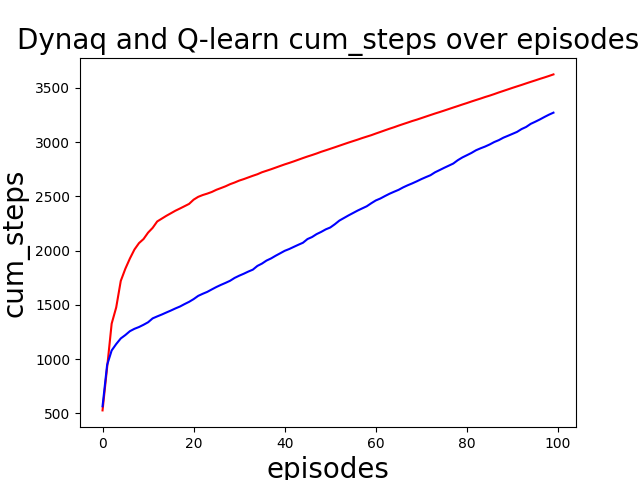
\includegraphics[scale=1.0]{Figure1.png}

\item
In the case where the environment switches from "Taxi-v4" to "Taxi-v5" after the initial 100 episodes, the length of each episode drastically increased as the algorithm needed more iterations to adjust the model and action-values to the new environment. As the algorithm was able to iterate and better learn the new environment, the length of each episode begins to converge to a constant as represented by a straight line. In order to better account for the change in the environment, I have modified the use of the algorithm to use a lower discount rate ($\gamma$). In my case, I used a discout factor of 0.5, which would help in a faster adjustment to the new environment by reducing the weight placed on already learned Q values. As a result, the algorithm is affected less by future expected returns and more by the immediate rewards, which greatly boosts immediate learning to a changing environment. Note that a similar change can be seen by decreasing alpha, the step size, as well as a combination of both.

The plot below displays this difference with the two curves. The red curve is the original algorithm prom part (a) reacting to the change in the environment. The blue curve represents the modified algorithm as described above.

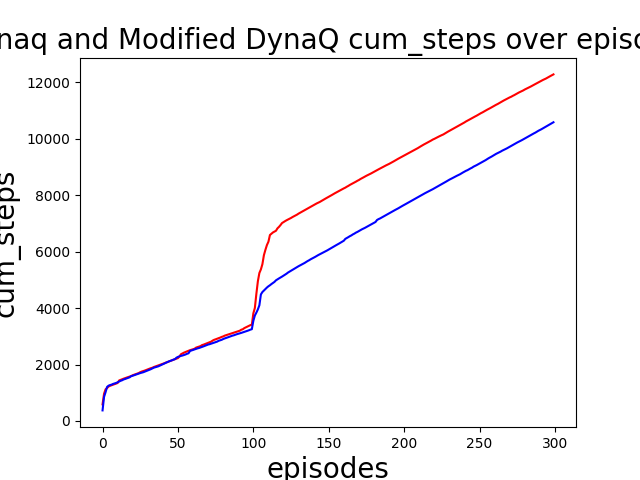
\includegraphics[scale=1.0]{Figure2.png}
\end{enumerate}

\section*{Question 2}
Below is the plot produced in an attempt to reproduce the right plot in Figure 9.2 of the textbook.

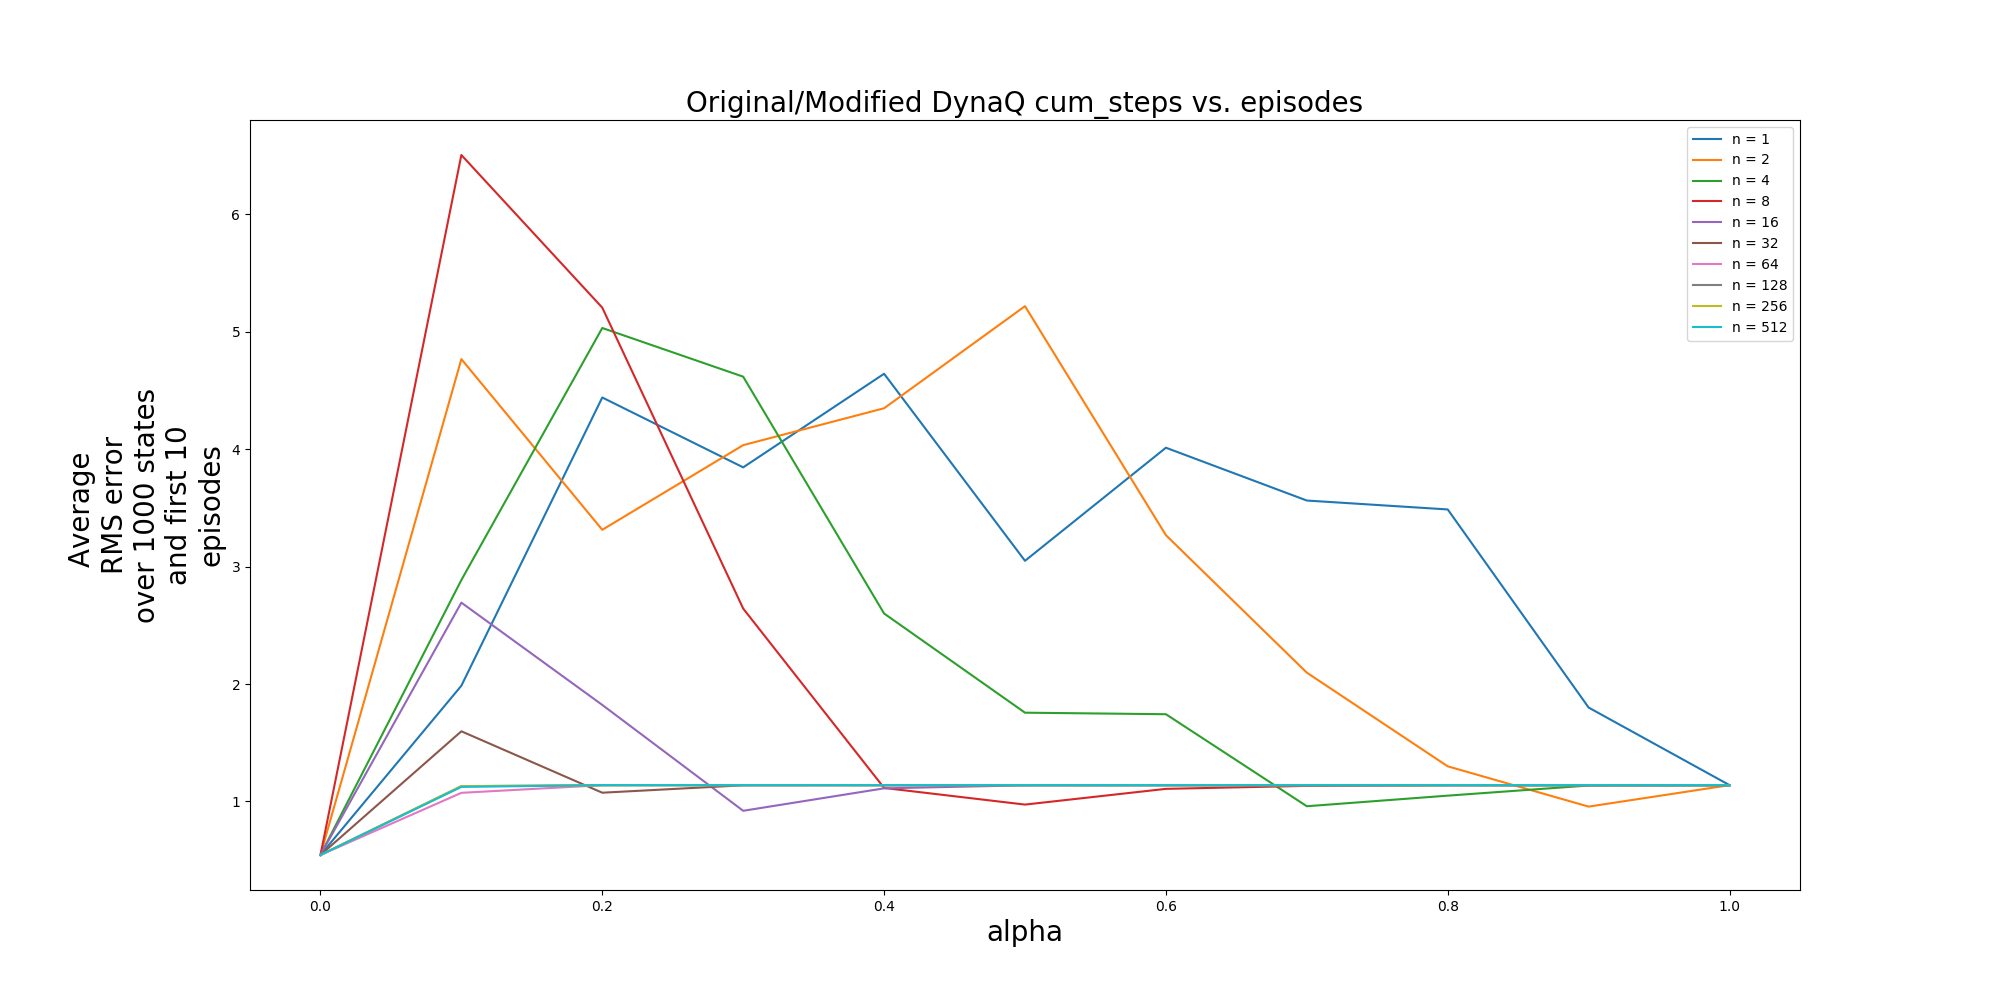
\includegraphics[scale=0.35]{FigureY.png}

\section*{Appendix: Relevant Code - tjha.py}
\lstinputlisting[language=Python, breaklines=true, numbers=left]{tjha.py}   
\end{document}
